% ===========================================================================
%
%		FEDERICO II THESIS TEMPLATE - ENGLISH
%  					* an example of Chapter 1: information about the discussion of the thesis
%	 
% 		AUTHOR:  		Antonio Esposito (antonio.esposito103@studenti.unina.it)
%		LAST UPDATED:	2017/06/20
%
% ===========================================================================

\chapter{Modello di Dominio}

%%%%% ===============================================================================
%\section{Classi, oggetti e relazioni di analisi}

%%%%% ===============================================================================
\section{Diagrammi di sequenza di analisi}
Si riportano di seguito i diagrammi di sequenza di analisi.
\begin{figure}[h!]
    
\includegraphics[width=\textwidth]{SequenceAnalisi/1.png}
\end{figure}
\begin{figure}[h!]
    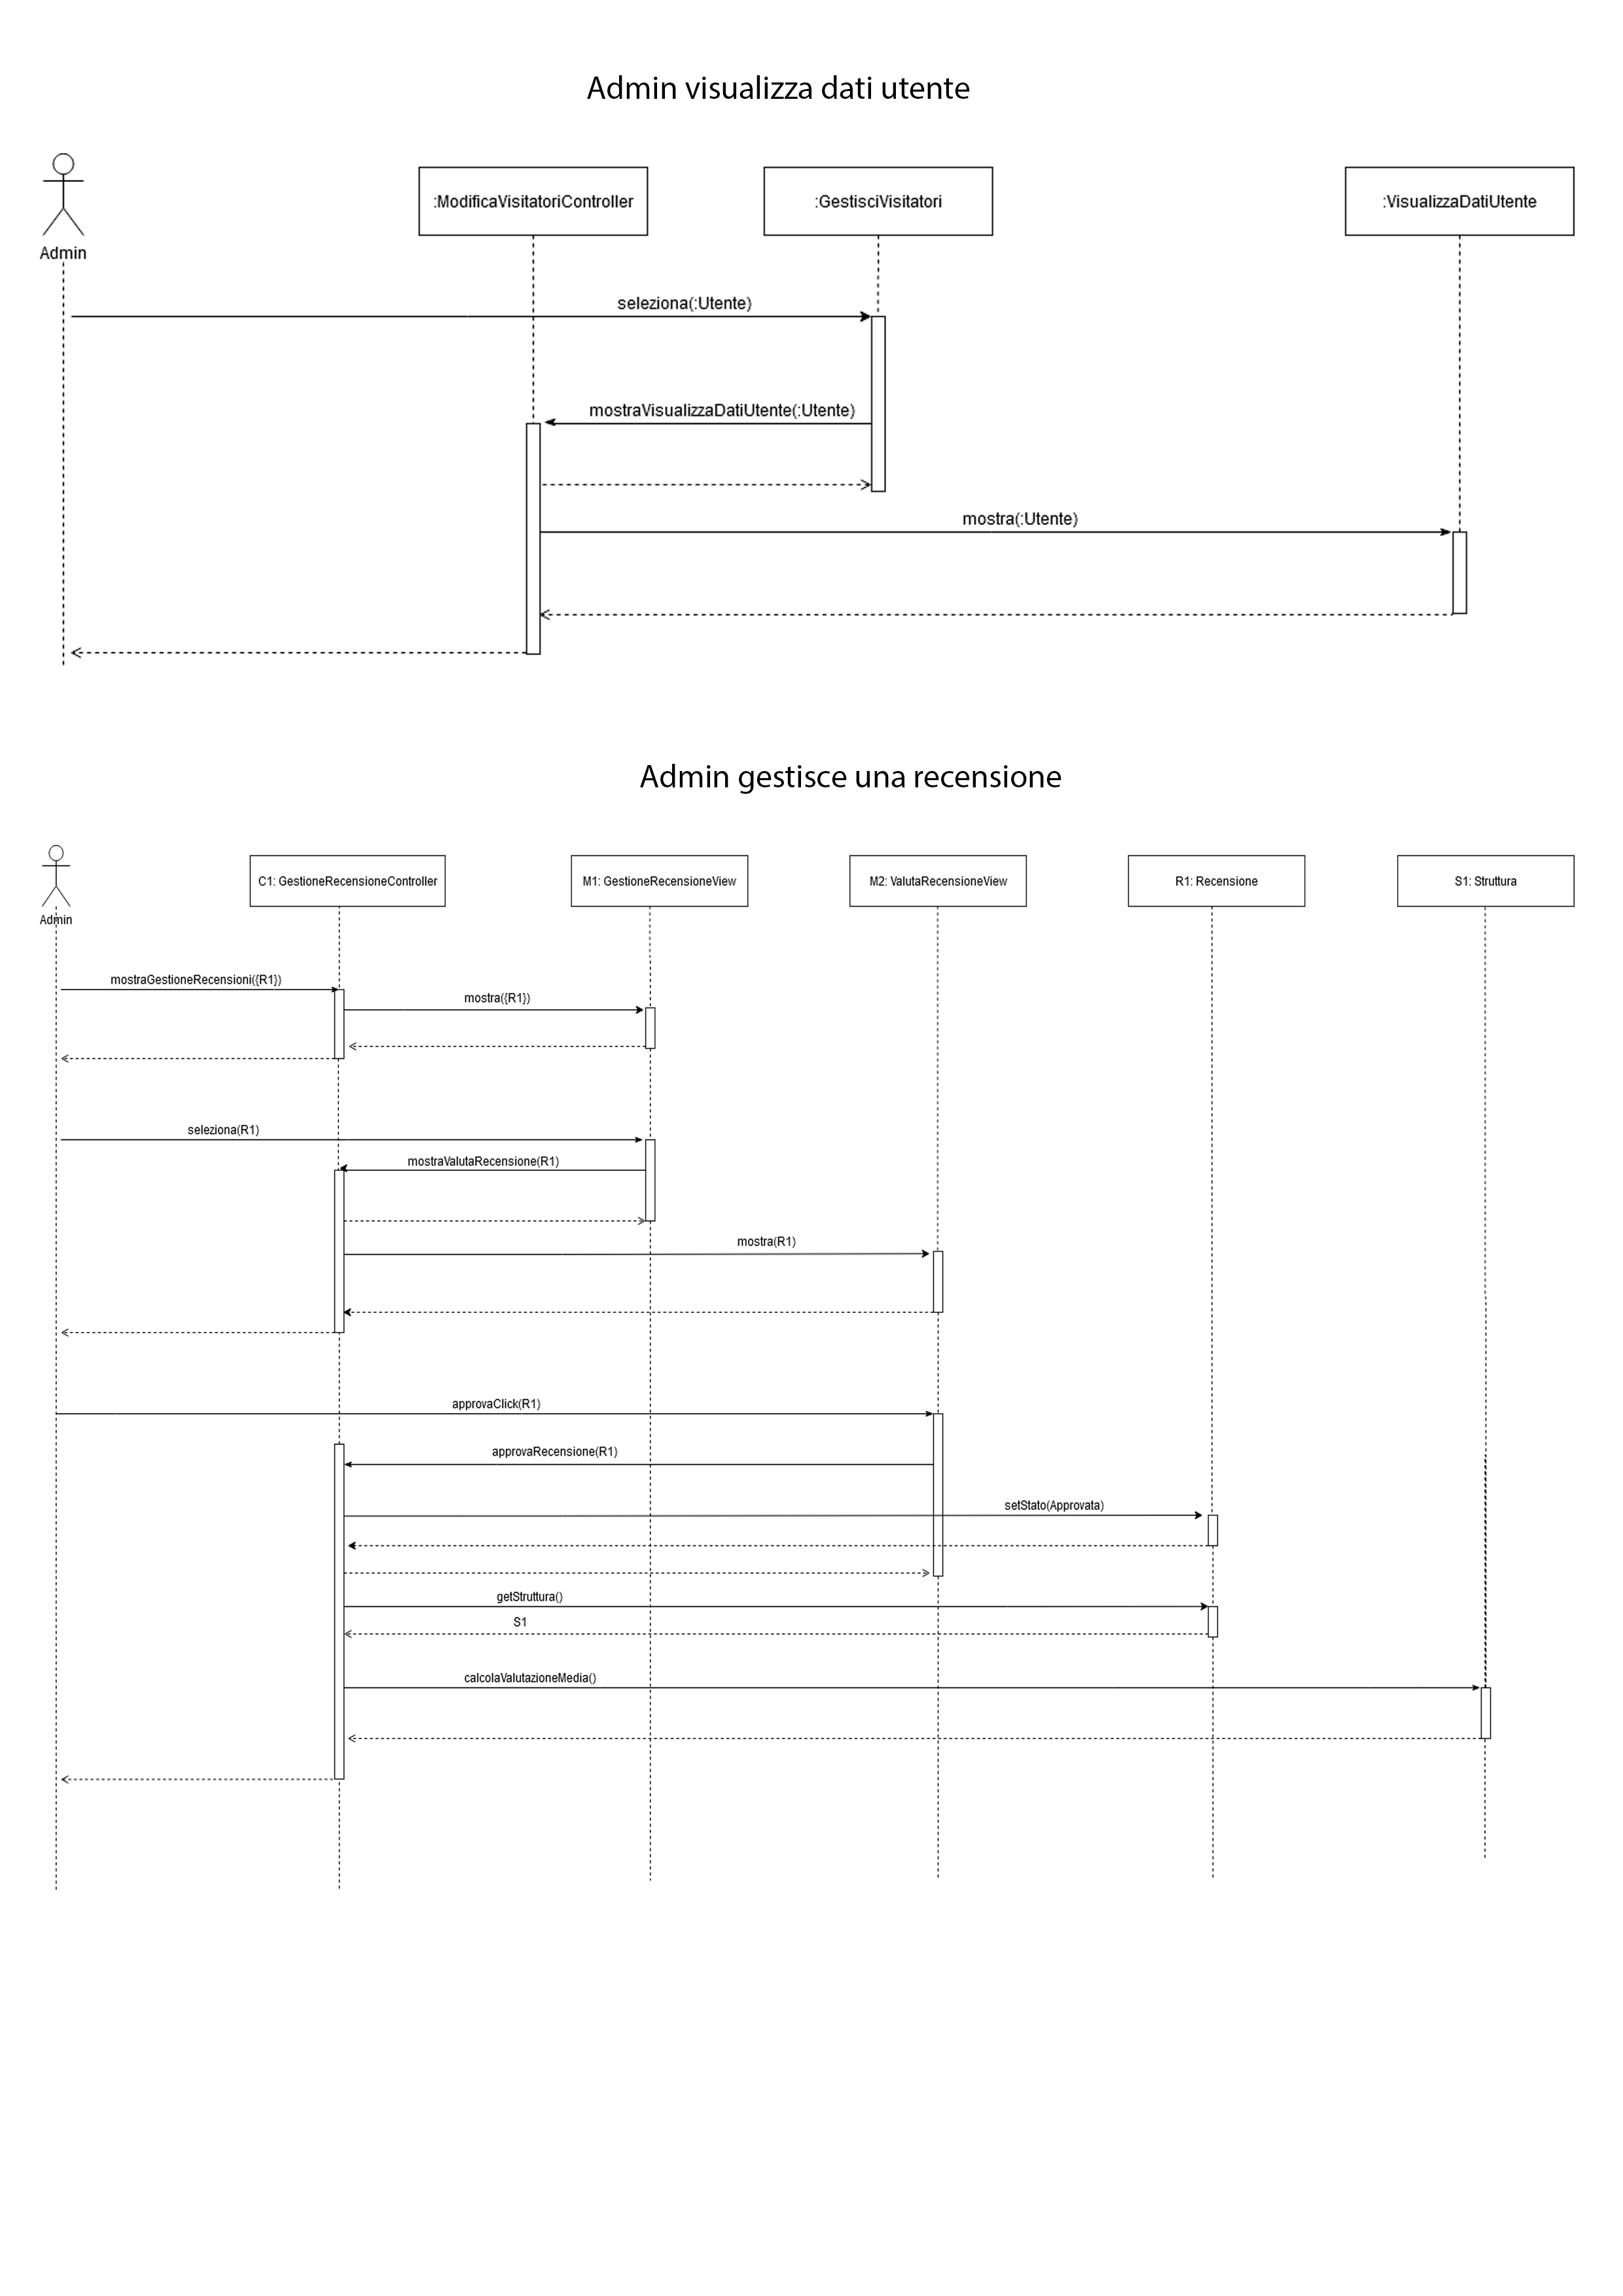
\includegraphics[width=\textwidth]{SequenceAnalisi/2.png}
\end{figure}
\begin{figure}[h!]
    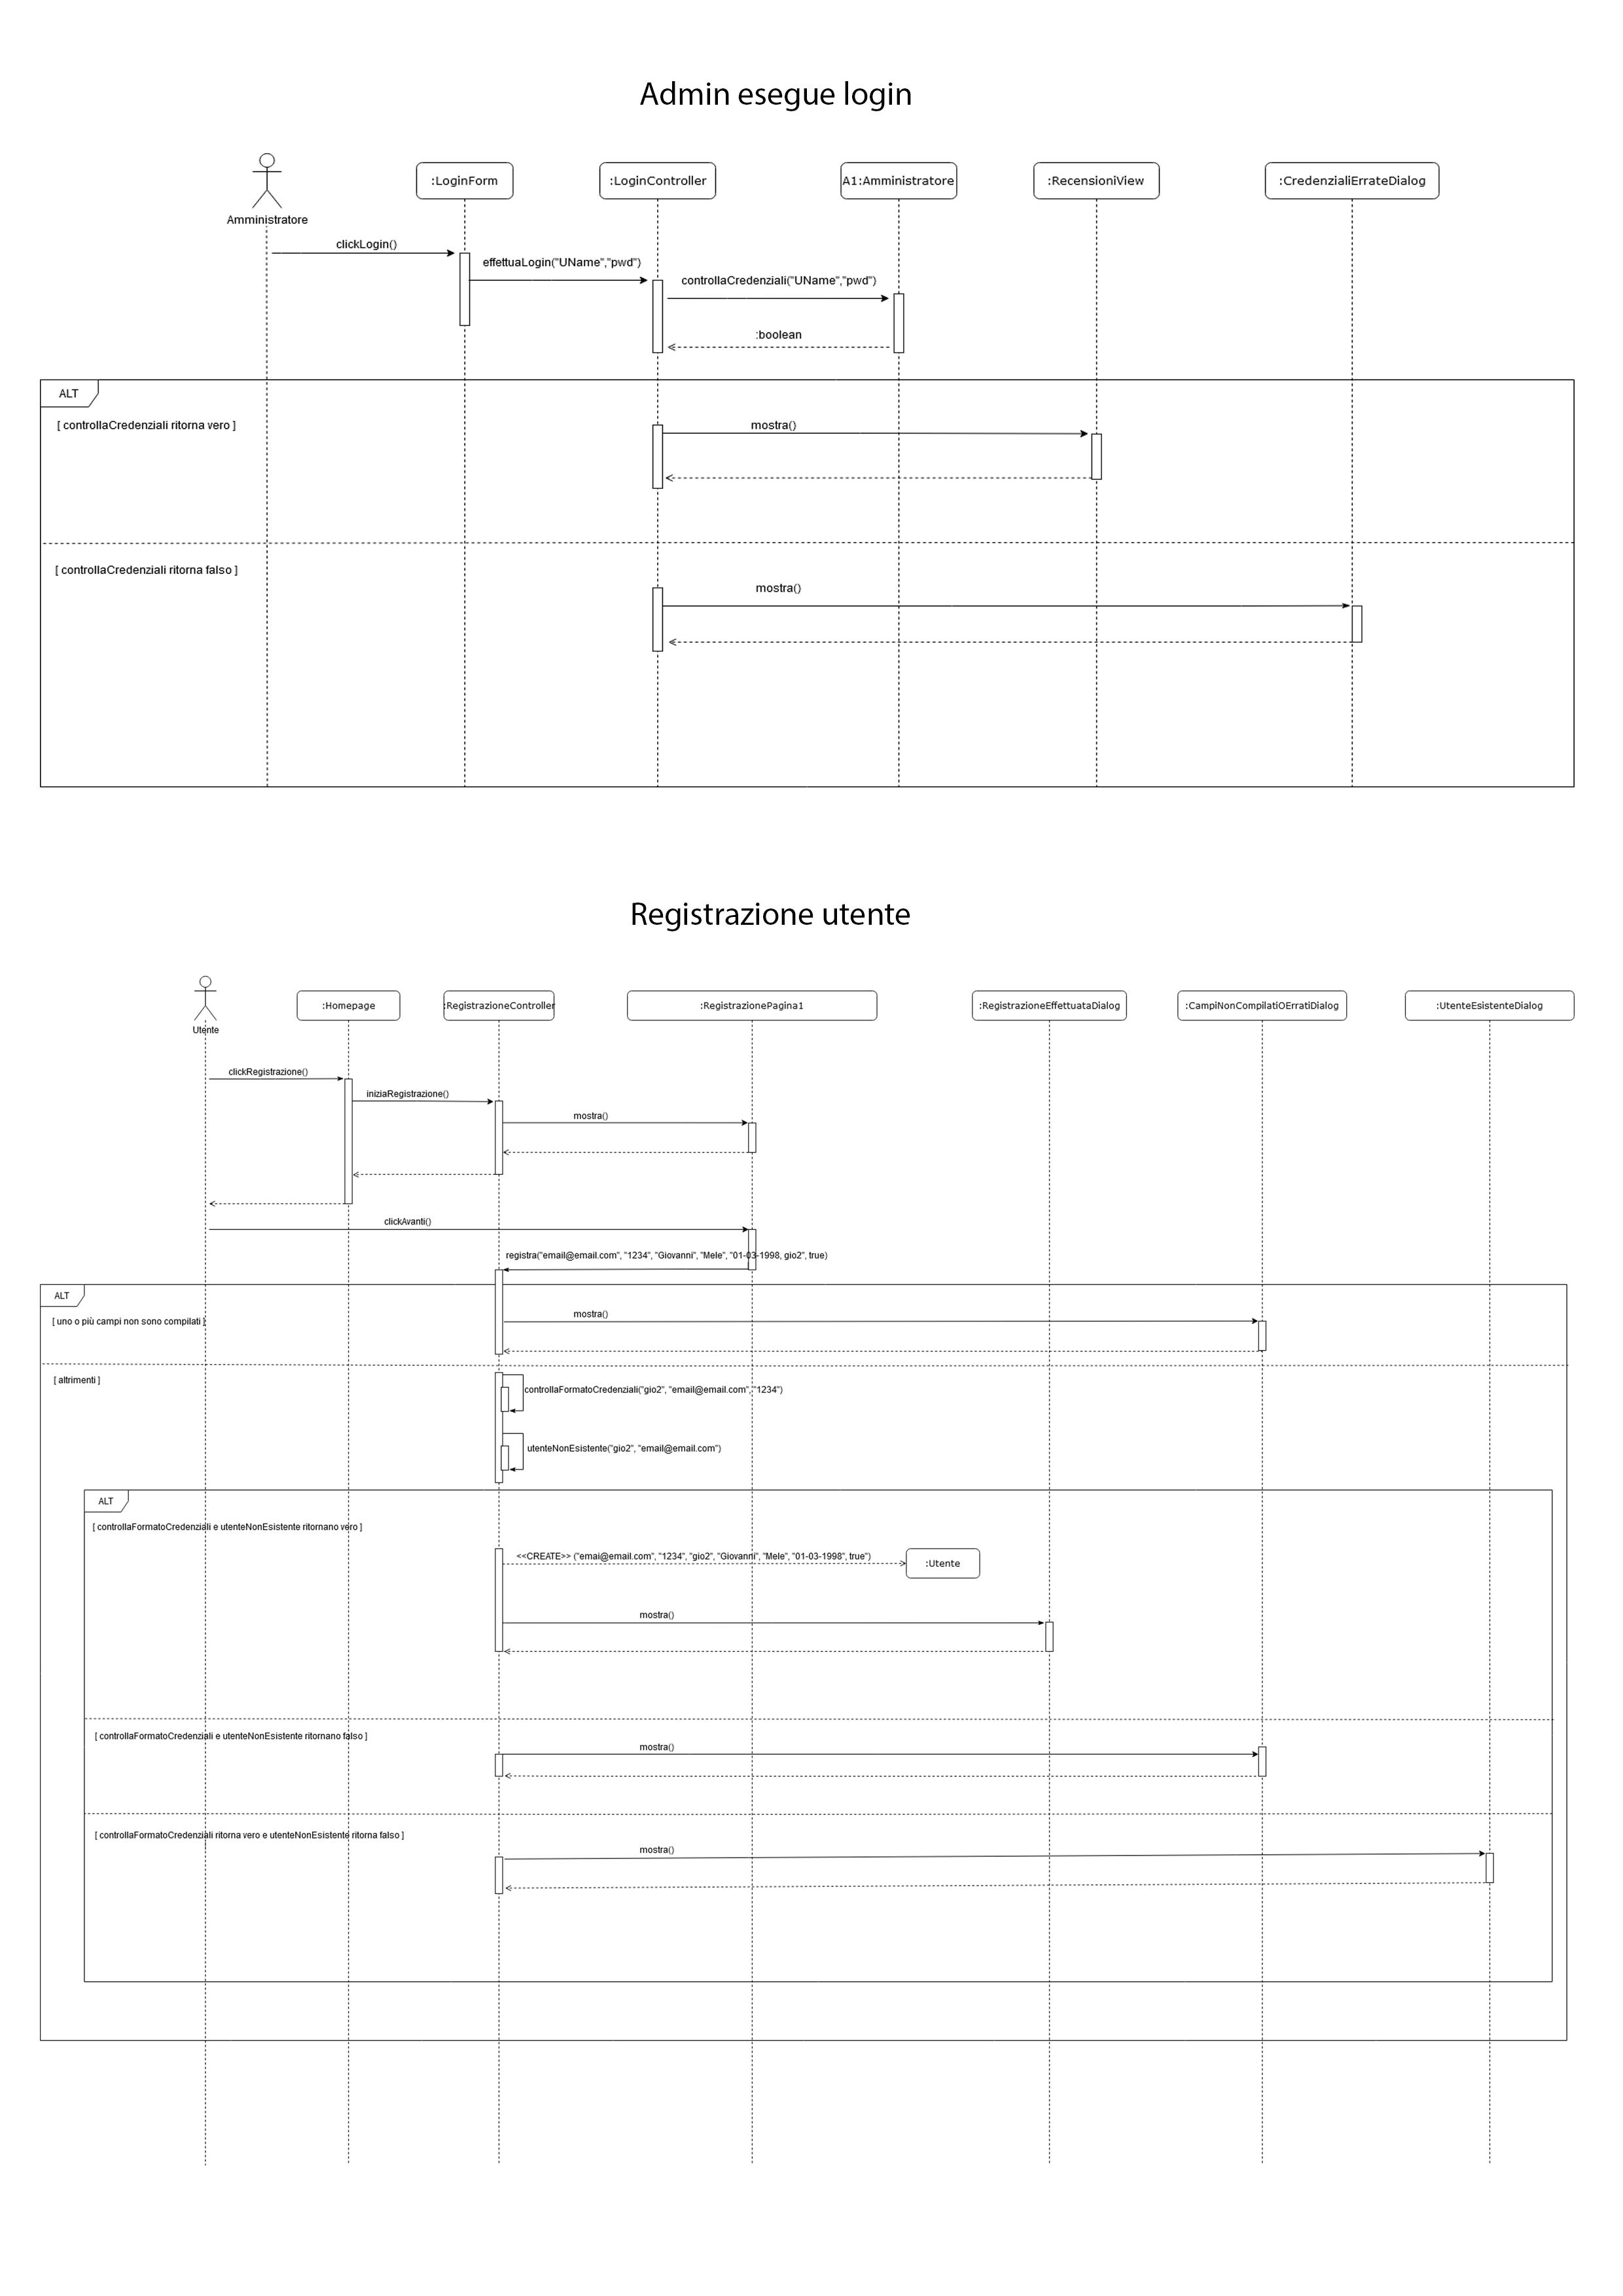
\includegraphics[width=\textwidth]{SequenceAnalisi/3.png}
\end{figure}
\begin{figure}[h!]
    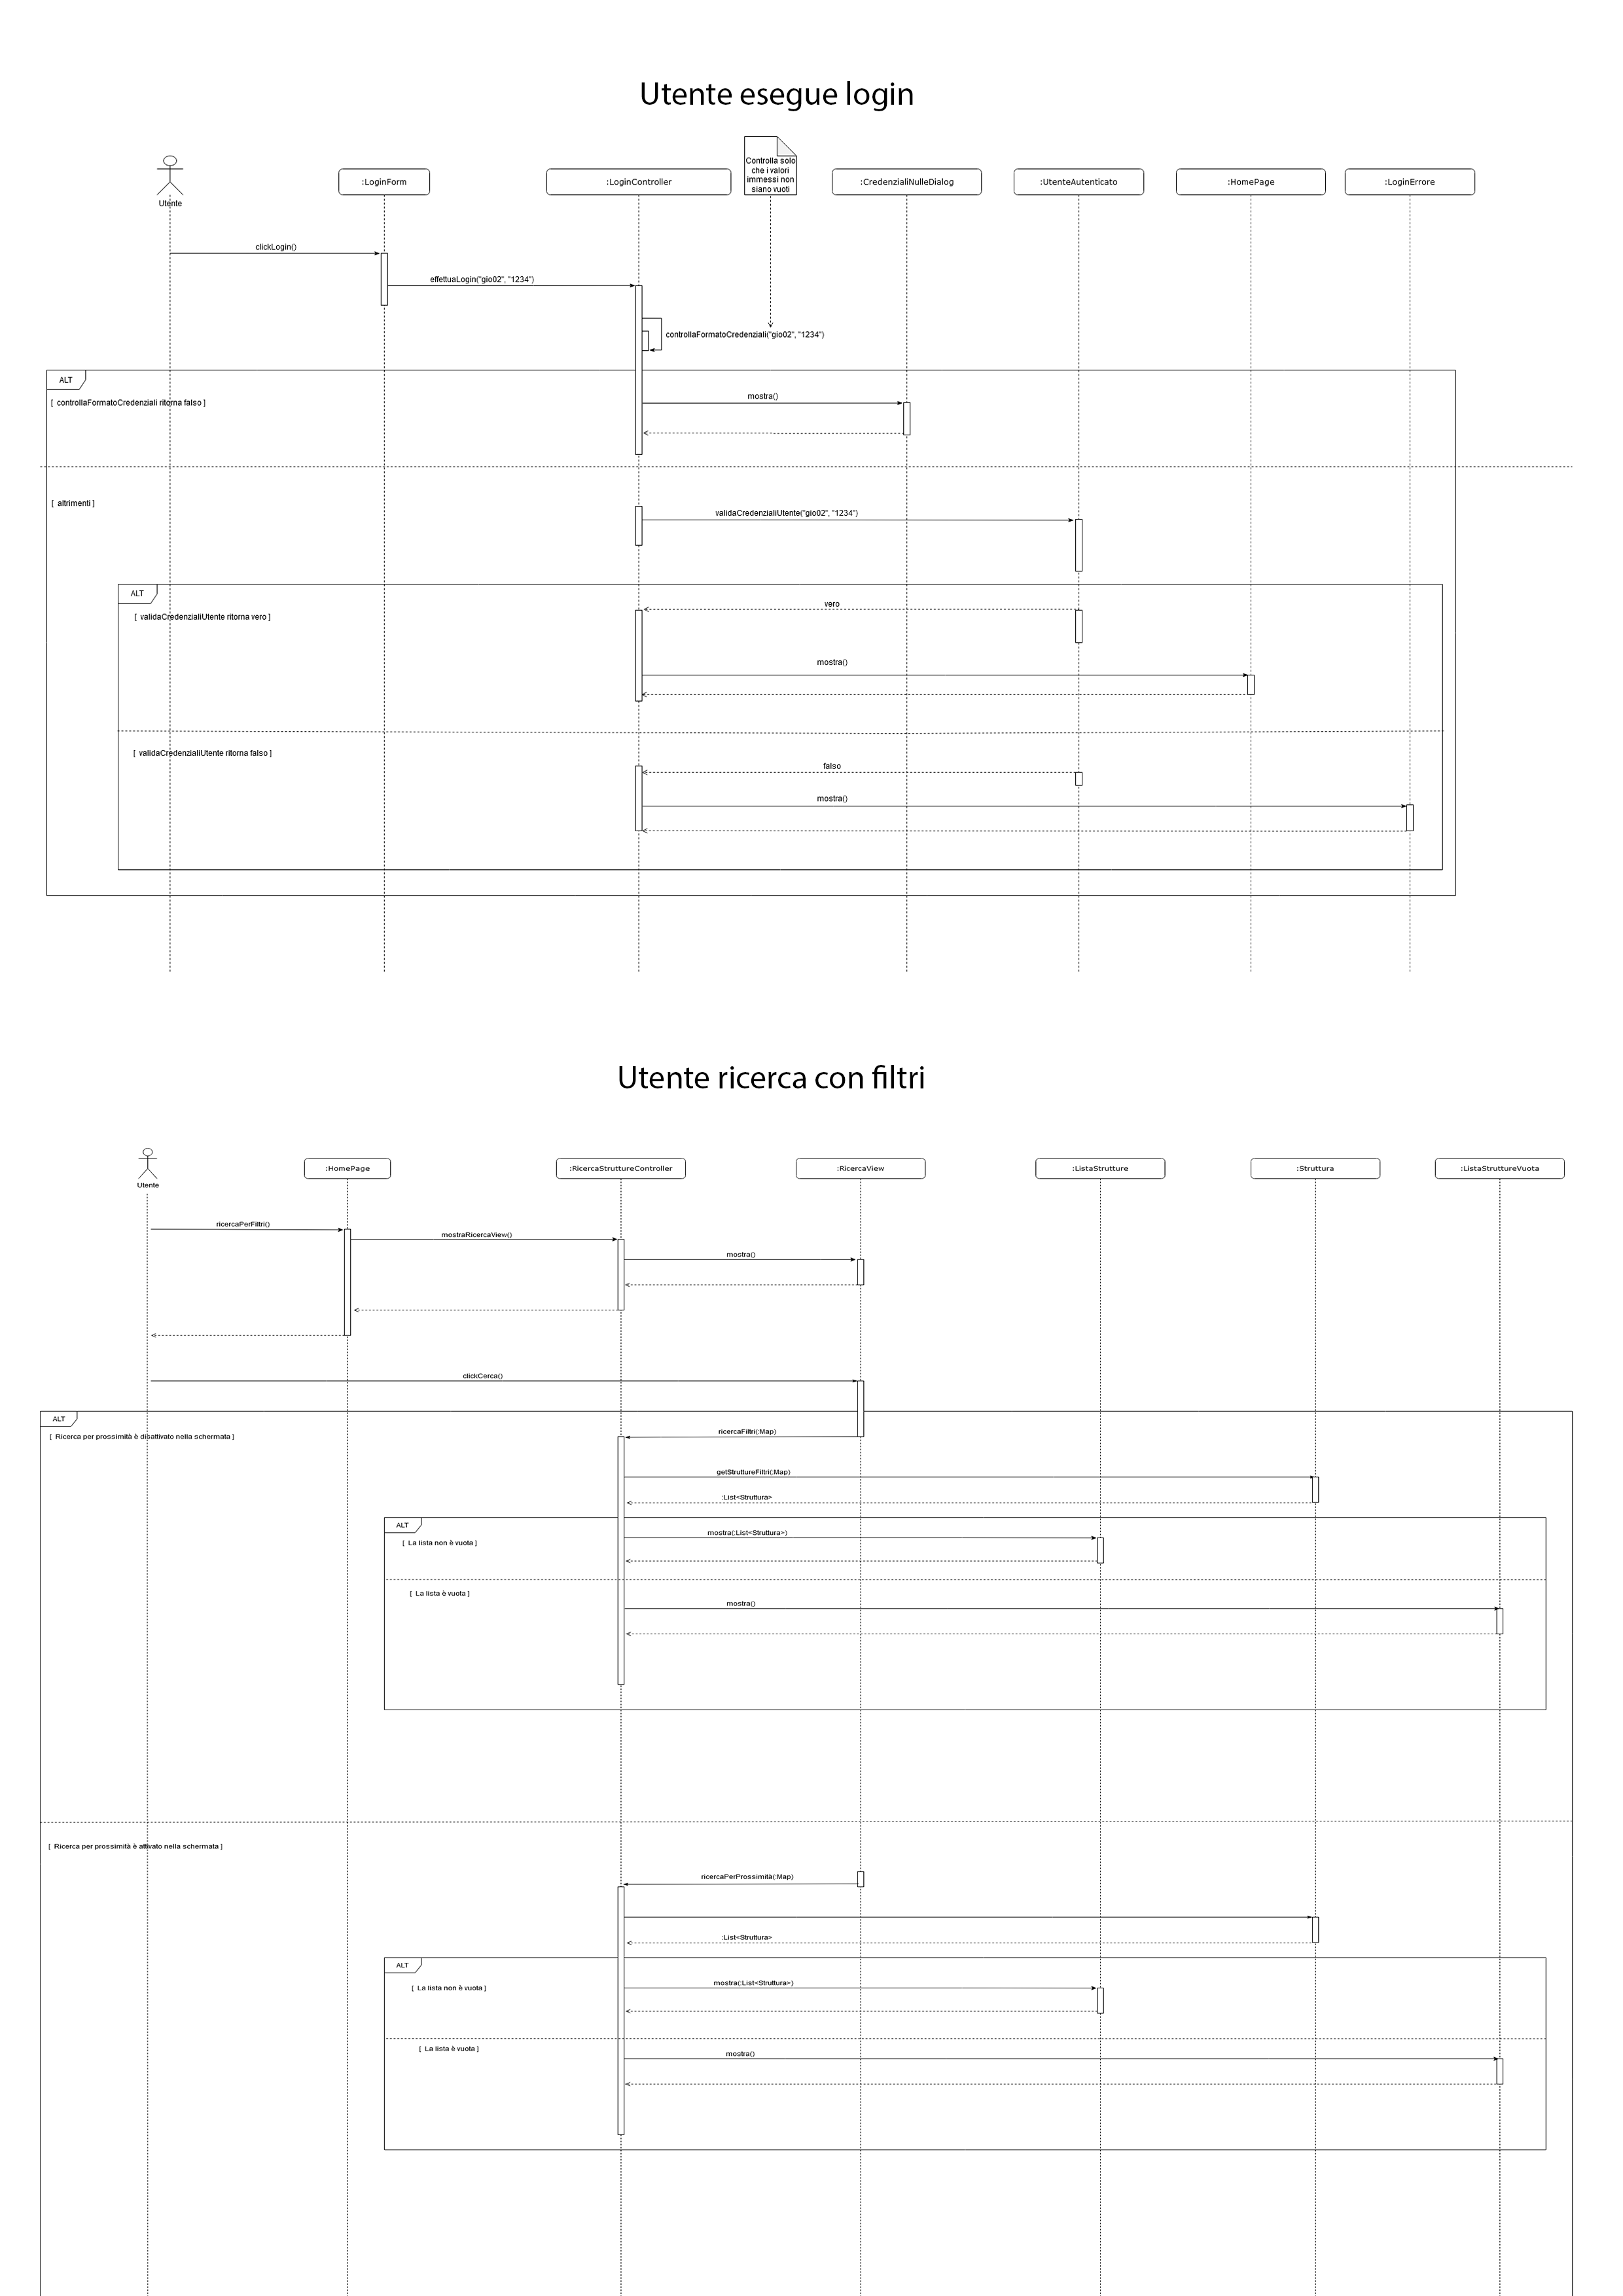
\includegraphics[width=\textwidth]{SequenceAnalisi/4.png}
\end{figure}
\begin{figure}[h!]
    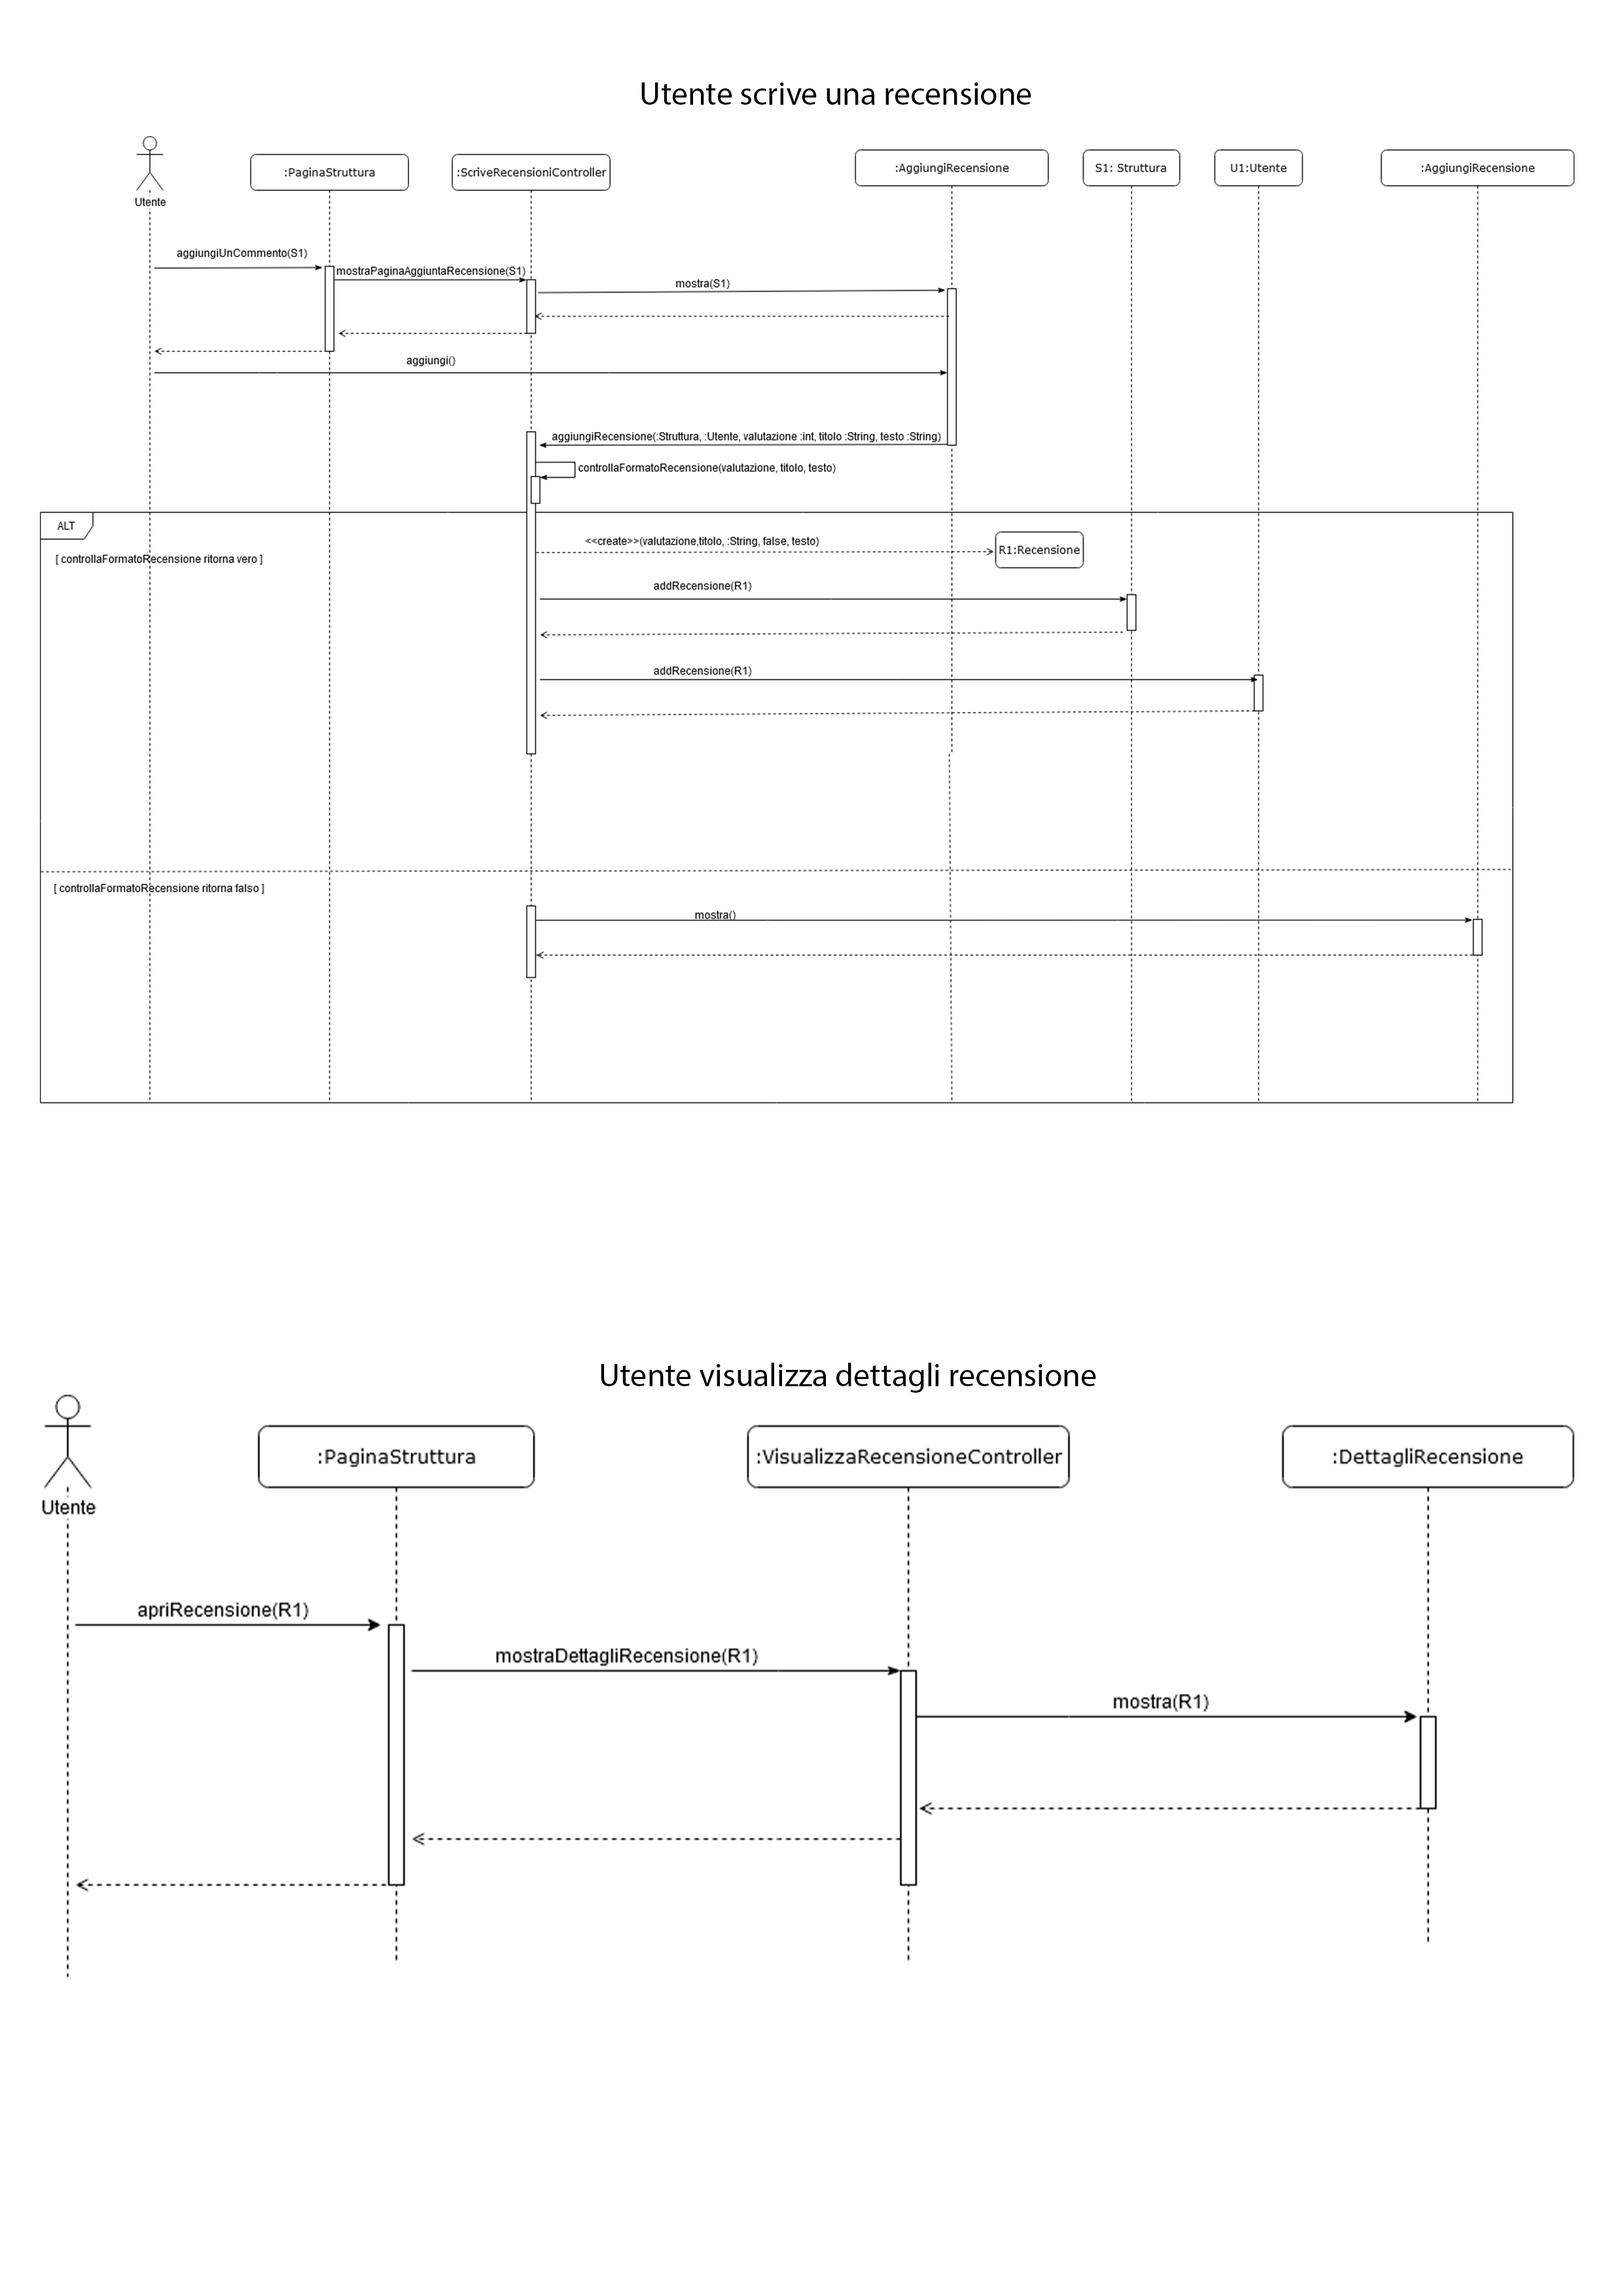
\includegraphics[width=\textwidth]{SequenceAnalisi/5.png}
\end{figure}
\begin{figure}[h!]
    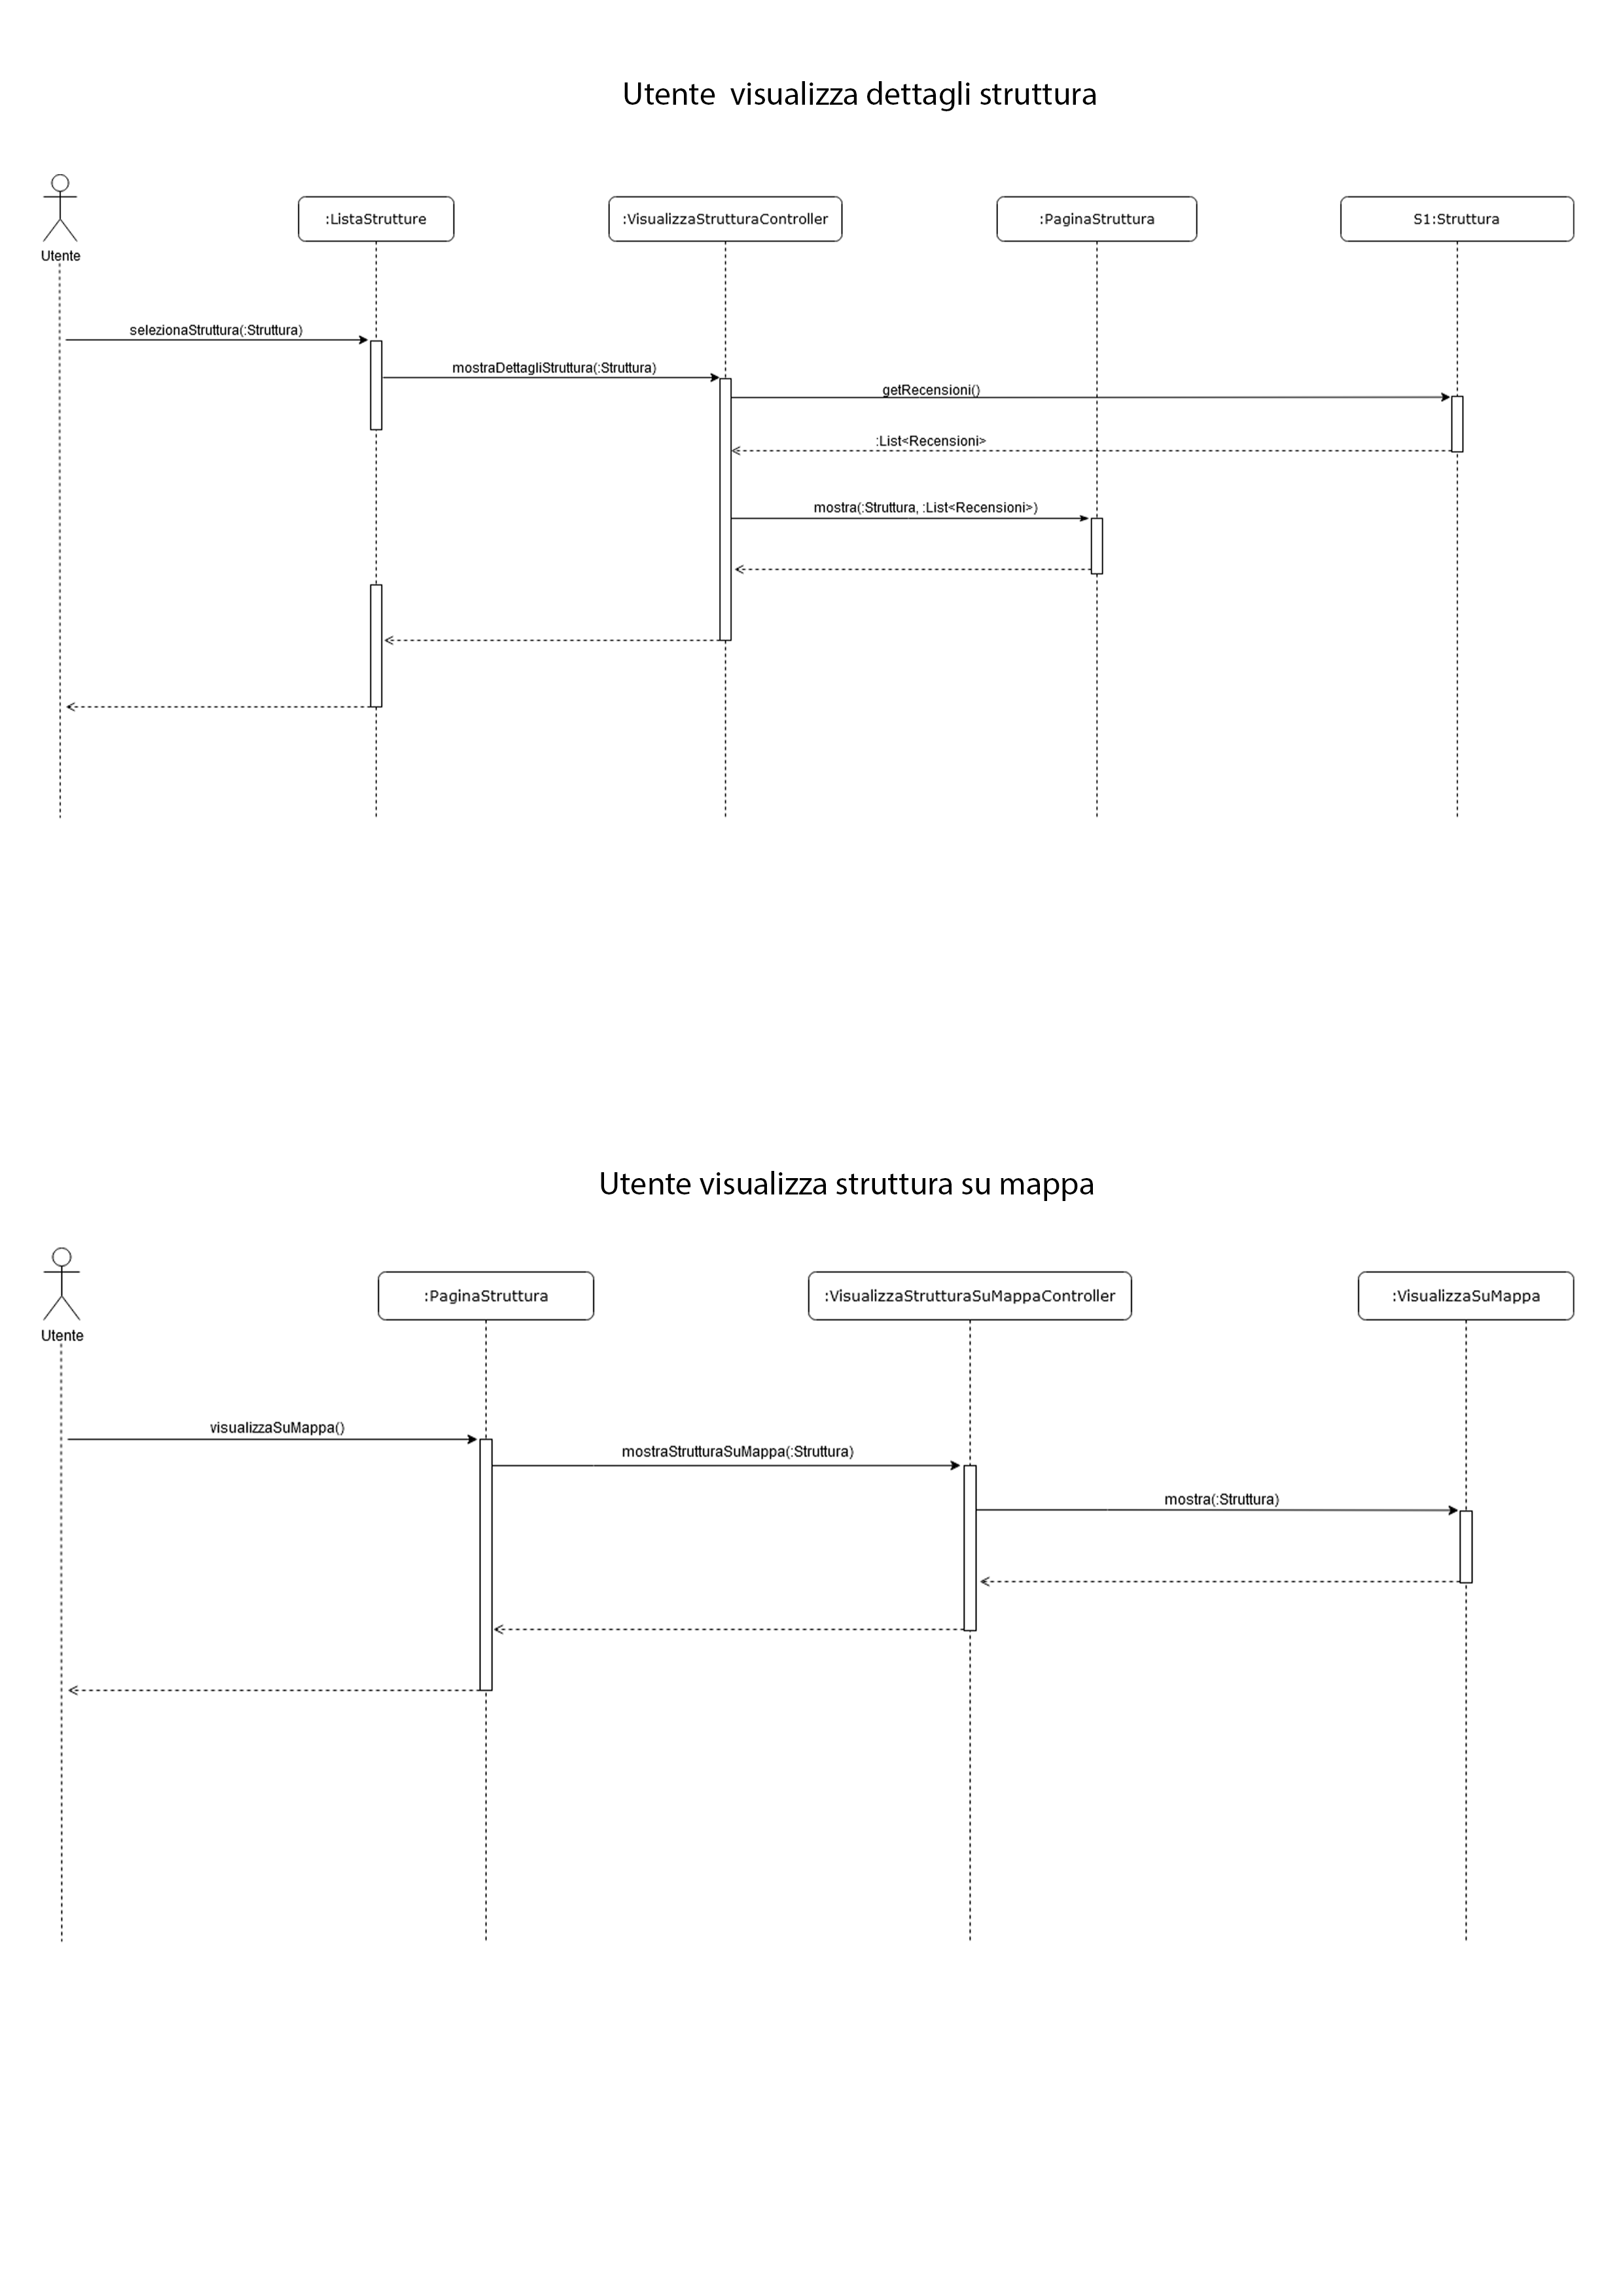
\includegraphics[width=\textwidth]{SequenceAnalisi/6.png}
\end{figure}
%%%%% ===============================================================================
\section{Diagrammi di stato di attività}


%%%%% ===============================================================================
\section{Diagrammi di attività}


%%%%% ===============================================================================
